% Chapter Template

\chapter{Literature Review} % Main chapter title

\label{Chapter2} % Change X to a consecutive number; for referencing this chapter elsewhere, use \ref{ChapterX}



\section{Coarse Grained Force Fields}

Molecular simulations can be carried out at different levels of description. The detailed atomistic level or \textit{ab initio}level is described by the laws of quantum mechanics. The system consists of a set of subatomic particulars in which Schrodinger's equation is solved for all of them. The next level is the atomistic description. It considers that the system is made up of atoms following the laws of statistical mechanics.  Force fields at this level are based on pair potentials with Coulombic charged sites, which account for the molecular interactions. The contributions due to to intramolecular interactions like bond-stretching, angle-bending and torsion are also usually accounted by these kind of force fields. When the scale of the simulations needs to be increased and the atomistic simulations become too computationally expensive, the coarse-grained (CG) description is more suited. It considers that the system is made up of pseudo atoms or beads that contain multiple atoms or an entire molecule. 

There is a obvious loss of information in grouping atoms, hence it is necessary to assure that the process of eliminating unnecessary or unimportant information ('coarse graining') doesn't affect the system's physical behavior. Ideally, the coarse gained model needs to have accuracy, transferability, robustness, and computational efficiency. In order to achieve these goals, the coarse grained force fields are usually developed by mapping the atomistic model to define the pseudo atoms which are formed similar functional groups. The level of coarse-graining also needs to be defined, up to 6 heavy atoms (non-hydrogen atoms) per bead in order to not lose important details and maintain isotropic representations of the beads \cite{shinoda2007,martini2007,hadley2012}. The CG force field can be parametrized following two different approaches: bottoms up and top down. The bottoms up approach uses information of a more detailed scale such as the \textit{ab initio} description or the atomistic description to obtain the information necessary to the parametrization. This method depends highly of the quality of the detailed model to succeed. Meanwhile, the top down methodology obtains the parameters from larger scales, like experimental thermodynamic properties or native-structure based properties. 

One of the first applications of coarse grained models is the study of protein folding \cite{levitt1975,levitt1976}. These earlier protein CG models were based on the structure of the molecule and they contributed for the knowledge of the physicochemical forces associated with protein folding and protein interactions \cite{koga2001}.  More recent, models focused on retaining the protein's chemical specificity. The Bereau and Deresmo model \cite{bereau2009} has a up to four-bead representation and was used in studies of protein folding and aggregation. However, this model still needs tuning to improve protein stability \cite{bereau2010}. The OPEP (Optimized Potential for Efficient Protein Structure Prediction) model \cite{opep2014,opep2015} has up to six-bead representation. It was used to investigate a variety of phenomena, ranging from protein folding to \textit{ab initio} peptide structure prediction \cite{opep2011,opep2009,opep20092}. Other CG protein models used in the literature are the Scorpion (solvated coarse-grained protein interaction)  \cite{scorpion2013}, the UNRES (united residue) \cite{unres2014} and the MARTINI model \cite{martini2013}. The later one is the most popular model for the CG modeling of membrane proteins \cite{martini20132}. The MARTINI model is also extensively used as CG model for water. This model represents four water molecules as one bead using a shifted Lennard Jones potential for the non bonded interactions. Though its extensive use, the MARTINI water model doesn't properly represent properties as interfacial tension and compressibility \cite{shinoda2010} and can freeze at room temperature \cite{winger2009,martini2007}, what makes necessary the use of anti-freeze agents during the simulations. This behavior can be explained by the high level of coarse graining (4:1), the lack of explicit charges and the use of the 12-6 potential. With the idea of improving the MARTINI model, \citeonline{chiu2010} used the Morse Potential, which is softer than the LJ potential. Meanwhile, \citeonline{shinoda2007} used different forms of the Mie potential. They concluded that a 12-4 Mie Potential was ideal for the all water cross interactions and  a 9-6 Mie Potential was suited for all the solute-solute interactions. 

Outside of the Martini framework, \citeonline{shinoda2010} studied different levels of coarse-graining for water ranging for one to 4 molecules per bead using different Mie and Morse potentials. Other works also assessed the use of Soft-core potentials to study aqueous solutions of surfactants \cite{shinoda2007}, ionic liquids \cite{bhargava2009}, lipids \cite{shinoda20102} and membranes \cite{pantano2009}. Other CG force field for water based on the Mie Potential is the SAFT-$\gamma$ Mie \cite{lobanova2015}. In this model, the water molecule can be represented by two different one isotropic bead interacting via a 8-6 Mie Potential models. The CGW1-vle model was parametrized using saturated-liquid density and vapor pressure data, and should be used for simulations of aqueous systems' fluid-phase equilibrium at high temperatures and pressures. This model still suffers from premature freezing with a triple point at 343 K. The other model, CGW1-ift, was parametrized using saturated-liquid density and vapor-liquid interfacial tension, hence it is best suited for interfacial properties calculations. Both models have temperature-dependent size and energy parameters and performed well for these properties over the entire temperature range of the liquid. The SAFT-$\gamma$ Mie force field have also been applied to other compounds with satisfactory results. \citeonline{muller2017} parametrized the force field for aromatic compounds and tested it with simulations of fluid phase equilibrium. \citeonline{herdes2015} carried out simulations of alkanes and light gases with this force fields. Binary and ternary mixtures of water, carbon-dioxide and water \cite{lobanova2016}, thermodynamic and transport properties of carbon dioxide and methane \cite{cassiano1,cassiano2} and water/oil interfacial tension \cite{herdes2017} were also studied with this force field.   

%----------------------------------------------------------------------------------------
%	SECTION 2
%----------------------------------------------------------------------------------------



\section{Solvation Free Energies Based on Molecular Dynamics}

Free energies can be expressed as averages over ensembles of atomic configurations generated using Monte Carlo or molecular dynamics techniques. In the canonical ensemble, the free energy is given by:  

\begin{equation}
\label{eq:fcano}
\begin{aligned}
F(N,V,T) = -\kappa_{b}T ln Q(N,V,T)
\end{aligned}
\end{equation}
where $Q(N,V,T))$ is the partition function of the canonical ensemble:

\begin{equation}
\label{eq:partican}
\begin{aligned}
Q(N,V,T) = \int d^{n}p d^{n}r \exp \left[ -\beta \left( \sum_{i=1}^{N}\dfrac{p_{i}^{2}}{2m_{i}} + U(r_{1},..,r_{n}) \right)
\right]
\end{aligned}
\end{equation}
where $\beta=1/k_{b}T$. Meanwhile, the average over the isothermal-isobaric ensemble gives the Gibbs free energy:

\begin{equation}
\label{eq:fisobari}
\begin{aligned}
G(N,P,T) = -\kappa_{b}T ln \Delta (N,P,T)
\end{aligned}
\end{equation}
where $\Delta (N,P,T)$ is the partition function of the isothermal-isobaric ensemble:

\begin{equation}
\label{eq:partiso}
\begin{aligned}
\Delta (N,P,T) = \frac{1}{V_{0}} \int_{0}^{\infty} dV \int d^{n}p d^{n}r \exp \left[ -\beta \left( \sum_{i=1}^{N}\dfrac{p_{i}^{2}}{2m_{i}} + U(r_{1},..,r_{n}) + PV(r_{1},..,r_{n}) \right) \right]
\end{aligned}
\end{equation}

Since it is only possible to obtain free energy differences, solvation free energy calculations based on molecular dynamics estimate the difference between the Gibbs free energies of end states:

\begin{equation}
\label{eq:dif}
\begin{aligned}
\Delta G_{AB} = G_{B} - G_{A}= -\kappa_{b}T ln \left( \frac{\Delta_{B}}{\Delta_{A}}\right) = -\kappa_{b}T ln \left( \frac{Z_{B}}{Z_{A}}\right)
\end{aligned}
\end{equation}

Since both states are at the same temperature, the moment integrals in the ratio ${\Delta_{B}}/{\Delta_{A}}$ can be simplified. Hence this ratio becomes equal to the ratio of configuration partition functions:

\begin{equation}
\label{eq:partiso}
\begin{aligned}
\dfrac{Z_{B}}{Z_{A}} = \dfrac{\int_{0}^{\infty} dV \int d^{n}r \exp \left[ -\beta \left(U(r_{1},..,r_{n}) + PV(r_{1},..,r_{n}) \right)_{B} \right]}{\int_{0}^{\infty} dV \int d^{n}r \exp \left[ -\beta \left(U(r_{1},..,r_{n}) + PV(r_{1},..,r_{n}) \right)_{A} \right]}
\end{aligned}
\end{equation}

The Gibbs free energy difference between end states $A$ and $B$ are, more specifically, the difference between the solute alone in the gas phase and the solute interacting with the solvent. In order to these differences be accurate, the sates' phase integral must have sufficient overlap  \cite{klimovich}. This can be achieved by calculating the free energy difference between a series of intermediates states. The result of these differences are independent of the path chosen since the free energy is a state function. That's why the states used typically don't have a physical sense, they are alchemical states which are only linking the physical states of interest. The strategy for solvation free energy calculations follows a thermodynamic cycle to gradually insert the solute molecule into the solvent as illustrated in the \figref{thermcy}. According to this cycle, the free energy of solvation can be expressed as:

\begin{equation}
\label{eq:freesolv}
\begin{aligned}
\Delta G_{solv} = \Delta G_{1 \rightarrow 4} = \Delta G_{1 \rightarrow 2} + \Delta G_{2 \rightarrow 3} + \Delta G_{3 \rightarrow 4}  
\end{aligned}
\end{equation}

\begin{figure}[th]
\centering
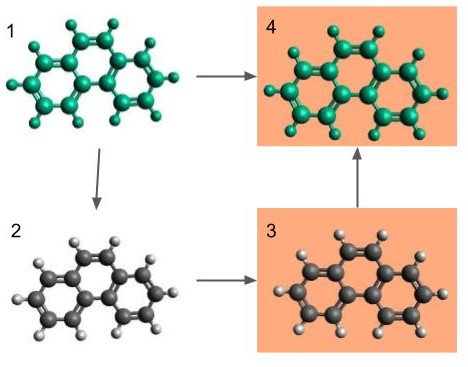
\includegraphics[scale=0.6]{Figures/cicclotermo.jpg}
\caption{Thermodynamic cycle for solvation free energy calculations with molecular dynamics (Adapted from \citeonline{klimovich})}
\label{thermcy}
\end{figure}

The solvation free energy between sates 1 and 2 in the cycle is the one associated with turning off the molecule's non bonded interactions in the gas phase. The following transformation, $\Delta G_{2 \rightarrow 3}$, is the free energy of moving the non-interacting molecule in the gas phase to the solvent and is equal to zero since the transformation of a non interacting molecule doesn't depend on the environment. Lastly, $\Delta G_{3 \rightarrow 4}$ is the free energy required to the  the non-interaction molecule in the aqueous phase regain its non-bonded interactions.  The solvation free energy calculation can be classified according to the types of the non bonded interactions that are turned of in the $1 \rightarrow 2$ and $ 3 \rightarrow 4$ parts of the cycle. If both the non-bonded interactions with the environment and the internal interactions are turned of, this is the annihilation free energy. Meanwhile, if only the non-bonded interactions with the environment are turned off,this is the decoupling free energy. In this later case, $\Delta G_{1 \rightarrow 2} = 0$ and the $\Delta G_{solv} = \Delta G_{3 \rightarrow 4} $. The methods used to carry out theses transformations scale the solute charges to zero and then turn of the interactions corresponding to the Lennard Jones potential. In order to carry out the later process, a modified potential with a coupling parameter $\lambda$ is used. Each $\lambda$ represent an alchemical state and, when $\lambda=0$, there is no interaction with the solvent and, when $\lambda=1$, the interactions are fully activated. The coupling of the $\lambda$ parameter could be linear, but it could generate numerical problems related to the exponential part of the Potential. That's why the non-linear soft-core scheme \cite{beutler1994} is usually used, the generalized soft core potential is given by:

\begin{equation}
\label{eq:softcore}
\begin{aligned}
U^{sc}(r) {}=& \lambda\epsilon\dfrac{\lambda_r}{\lambda_r - \lambda_a} \left(\frac{\lambda_r}{\lambda_a} \right)^{\left( \frac{\lambda_a}{\lambda_r - \lambda_a} \right)} \\
& \left\lbrace\dfrac{1}{\left[\alpha(1-\lambda)+ (r/\sigma)^{\lambda_a}\right]^{\lambda_{r}/\lambda_{a}}} - \dfrac{1}{\alpha(1-\lambda)+(r/\sigma)^{\lambda_a}}\right\rbrace
\end{aligned}
\end{equation}

Using the Lennard Jones exponents, Eq. \eqref{eq:softcore} becomes:

\begin{equation}
\label{eq:softcoreLJ}
\begin{aligned}
U_{LJ}^{sc}(r) {}=& 4\lambda\epsilon \left\lbrace\frac{1}{\left[\alpha(1-\lambda)+ (r/\sigma)^{6}\right]^{2}} - \frac{1}{\alpha(1-\lambda)+(r/\sigma)^{6}}\right\rbrace
\end{aligned}
\end{equation}

where $\alpha$ is a constant in which the value of 0.5 is normally assumed to it. The $\Delta G_{3 \rightarrow 4}$ can be then obtained by doing independent simulations in different values of $\lambda$ or by doing expanded ensemble simulations \cite{lyubartsev} which samples all state in a single simulation. This method allows a faster sampling across the alchemical states considering that the kinetic barriers are not substantial. 


\section{Post simulation methods}

The data obtained with molecular dynamics simulations method explained in the section above contain the potential energies correspondent to each $\lambda$. These potential energies obtained then needs to be post processed and analyzed in order to calculate the solvation free energies. Some of the widely used method for these calculations are going to be briefly describe below. 

\subsection{Thermodynamic integration}

The thermodynamic integration method \cite{kirkwood1935} uses equilibrium averages to evaluate the derivative of the potential energy with respect to the coupling parameter. Then, the free energies are obtained as the integration of the derivatives of the initial and final state:

\begin{equation}
\label{eq:ti}
\begin{aligned}
\Delta G_{solv} = \int_{0}^{1} \frac{\partial U}{\partial \lambda} d\lambda
\end{aligned}
\end{equation}

The integration in Eq. \eqref{eq:ti} is obtained by interpolating the output data form the simulations in different ways. Some examples of methods for the interpolations are the trapezoidal rule or natural cubic spline \cite{bareva}. There are also other more complex schemes that are usually system specific as the works of \citeonline{garrido2010} and \citeonline{shyu2009} and that use fitting functions to interpolate the data. 

\subsection{Free energy of Pertubation (FEP)}

The free energy of perturbation method \cite{zwanzig1954} is the oldest and one of the most general purpose strategy to calculate free energy differences. In this method, the difference between two thermodynamic states A and B is given by:

\begin{equation}
\label{eq:fep}
\begin{aligned}
\Delta G_{AB} = -\frac{1}{\beta} ln \langle{e^{-\beta (U_{B}-U_{A})}}\rangle_{A}
\end{aligned}
\end{equation}

According to the equation above, the free energy difference is calculated by doing an average over the potential energies of state A and B obtained during the simulation of state A. This method requires a great overlap between states, the state B needs to represent a small perturbation in state A, in order to obtain a rapid convergence of the free energy difference. To assure the overlap, it is possible to carry out simulations in N intermediate sates between A and B, so Eq. \eqref{eq:fep} becomes:

\begin{equation}
\label{eq:fepint}
\begin{aligned}
\Delta G_{AB} = -\frac{1}{\beta} ln \left(\frac{1}{N}\sum_{i=0}^{N+1}
{e^{-\beta (U_{i+1}-U_{i})}}\right)_{i}
\end{aligned}
\end{equation}

The way of calculating $\Delta G$ of Eq. \eqref{eq:fepint} is called Exponential Averaging (EXP) \cite{zwanzig1955,bareva}. The direction of the transformation is also important in this method. If the direction is of decreasing entropy, the step is of insertion ($\Delta G_{AB}$) and method is called insertion exponential averaging (IEXP). The direction of increasing entropy is  called a deletion step ($\Delta G_{BA}$) and the method is labeled as deletion exponential averaging (DEXP). These directions can yield different values of free energy differences due the under sampling in the tail regions of the $\Delta G_{AB}$ distribution \cite{klimovich,pohorille2010}. These problems makes the EXP methods not suited to calculate free energy differences when the system hasn't a sufficient a overlap. For these cases, the Bennet Acceptance Ratio or the Multi-State Bennet Acceptance Ratio is more indicated.   

\subsection{Bennet Acceptance Ratio (BAR)}

The BAR method \cite{bennet1976} was developed with the intent of eliminating the bias in the free energy estimation. It uses the uncorrelated samples of the potential energy in both directions ($A \rightarrow B$ and $B \rightarrow A$) to obtain the free energy differences using the information in a statically optimal way. The free energy difference between two intermediate states (i and j) is calculated by the self-consistence solution of the following equations: 

\begin{equation}
\label{eq:bar1}
\begin{aligned}
\Delta G_{ij} = \frac{1}{\beta} ln \left( \dfrac{\sum_{k=1}^{N_{j}} \dfrac{1}{1+\exp[-\beta(\Delta U_{k}^{j}-C)]}}{\sum_{l=1}^{N_{i}} \dfrac{1}{1+\exp[-\beta(\Delta U_{l}^{i}-C)]}}\right) + C - \frac{1}{\beta}ln\left(\frac{N_{j}}{N_{i}}\right)
\end{aligned}
\end{equation}

\begin{equation}
\label{eq:bar2}
\begin{aligned}
 C = \Delta G_{ij} + \frac{1}{\beta}ln\left(\frac{N_{j}}{N_{i}}\right)
\end{aligned}
\end{equation}

The total free energy difference between end states is then given by the sum over the differences of consecutive intermediate states. This method also provides a function to obtain the minimum variance for the free energy difference. The variance equation for any value of C is given by:

\begin{equation}
\label{eq:barvar}
\begin{aligned}
 s_{ij}^{2} = \frac{1}{\beta^{2} N_{i}} \left[\dfrac{\langle{f^{2}(x)}\rangle_{i}}{\langle{f(x)}\rangle^{2}_{i}} - 1\right] + \frac{1}{\beta^{2} N_{j}} \left[\dfrac{\langle{f^{2}(x)}\rangle_{j}}{\langle{f(x)}\rangle^{2}_{j}} - 1\right]
\end{aligned}
\end{equation}
where $f(x)=1/(1+x)$ is the Fermi equation and $x=\exp[\beta(\Delta U - C)]$. The variance of the free energy difference between end sates can be calculated by assuming independent errors and summing over the variance of consecutive intermediate states. However, this assumption is not correct and there is no general formula to obtain a statistically unbiased estimate of an entire transformation with the BAR method \cite{bareva}. 

There are tow other methods related to the BAR method that don't solve the Eqs. \eqref{eq:bar1} and \eqref{eq:bar2} self consistently. By doing that, the free energy difference will not have minimum variance, but significant space and disk memory can be saved since the averages of Eqs. \eqref{eq:bar1} - \eqref{eq:barvar} are accumulated.The two methods are the Unoptimized Bennett Acceptance Ratio (UBAR) and Range-Based Bennett Acceptance Ratio (RBAR). The first one avoids the self consistently resolution of the BAR equations by defining $C=\beta^{-1}ln(N_{j}/N_{i})$. The UBAR method requires that the intermediate free energies differences are approximately equal to zero to obtain optimal estimations. Meanwhile, the RBAR method selects a range initial guesses of the constant $C$ in order to calculet a range  of $\Delta G_{ij}$. The value of free energy difference correspondent to the minimum variance is then used as input in Eq. \eqref{eq:bar2} to calculate the value of $C$. Hence, this method requires a good estimation of the initial range of the values of $C$. IN therms of accuracy, the UBAR method can be as accurate as the BAR method, but it may end up being as computational costly \cite{bareva}.  

\subsection{Multistate Bennet Acceptance Ratio (MBAR)}\label{mbar}

The MBAR method \cite{mbar} is a further development of the BAR method. The method proposes a estimator that computes free energies and their uncertainties of all the $K$ states  by minimizing the $KxK$ matrix of variances simultaneously. The estimator solves self consistently for each $G_{i}$ the following equation:

\begin{equation}
\label{eq:mbar}
\begin{aligned}
 G_{i} = \frac{1}{\beta}ln \sum_{k=1}^{K} \sum_{n=1}^{N_{k}}
 \dfrac{\exp[-\beta U_{i}(x_{kn})]}{\sum_{l=1}^{K} N_{l} \exp[\beta (G_{l} - U_{l}(x_{kn}))]}
\end{aligned}
\end{equation}

The equation above requires that the potential energy  of uncorrelated configuration $n$ to be evaluated for all K states ($U_{i}(x_{kn}$) and for all the uncorrelated configuration snapshots ($N_{k}$) from state $k$. The free energy change between the states is given then by $\Delta G_{ij} = G_{j} -  G_{i}$. The statistical variance of $S_{ij}^{2} \Delta G_{ij}$ is given by the matrix covariances:

\begin{equation}
\label{eq:varmbar}
\begin{aligned}
 s_{ij}^{2} \Delta G_{ij} \equiv cov (-ln \hat{Z_{j}}/\hat{Z_{i}},-ln \hat{Z_{j}}/\hat{Z_{i}})
\end{aligned}
\end{equation}
where $\hat{Z_{j}}$ and $\hat{Z_{i}})$ are the partition functions of states $i$ and $j$. The MBAR method can be considered as limit case of the 
weighted histogram analysis method (WHAM) \cite{wham} for computing free energies. The Eq. \eqref{eq:mbar} becomes equal to the WHAM equations if the histogram width tend to zero. Despite this, the MBAR is still more suited because it doesn't have the bias associated with the discretization  and it allows to calculate an error estimate.

